% Tukey plot
% Author: Sivaram Neelakantan
\documentclass[tikz, border=10pt]{standalone}
\usepackage{tikz}
\usetikzlibrary{arrows,backgrounds,snakes}
\begin{document}

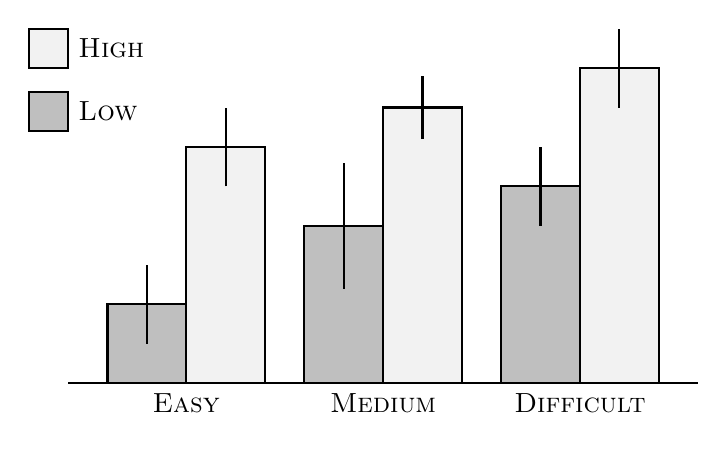
\begin{tikzpicture}[thick]
    \filldraw[fill=gray!50] (1,0) rectangle (2,1);% draw the box
    \draw (1.5,0.5) -- (1.5,1.5);
    \filldraw[fill=gray!10] (2,0) rectangle (3,3);% draw the box
    \draw (2.5,2.5) -- (2.5,3.5);
    \node[below] at (2,0) {$\textsc{Easy}$};


    \filldraw[fill=gray!50] (3.5,0) rectangle (4.5,2);% draw the box
    \draw (4,1.2) -- (4,2.8);
    \filldraw[fill=gray!10] (4.5,0) rectangle (5.5,3.5);% draw the box
    \draw (5,3.1) -- (5,3.9);
    \node[below] at (4.5,0) {$\textsc{Medium}$};


    \filldraw[fill=gray!50] (6,0) rectangle (7,2.5);% draw the box
    \draw (6.5,2) -- (6.5,3);
    \filldraw[fill=gray!10] (7,0) rectangle (8,4);% draw the box
    \draw (7.5,3.5) -- (7.5,4.5);
    \node[below] at (7,0) {$\textsc{Difficult}$};

    \filldraw[fill=gray!10] (0,4) rectangle (0.5,4.5);% draw the box
    \node[right] at (0.5,4.25) {$\textsc{High}$};
    \filldraw[fill=gray!50] (0,3.2) rectangle (0.5,3.7);% draw the box
    \node[right] at (0.5,3.45) {$\textsc{Low}$};


    % Axis
    \draw (0.5,0) -- (8.5,0);

\end{tikzpicture}

\end{document} 